\documentclass[11pt]{article}

\usepackage[paper=a4paper,dvips,top=4cm,left=2.5cm,right=2.5cm,
foot=2cm,bottom=4cm]{geometry}
%\usepackage{float}
\usepackage[linesnumbered,ruled,vlined]{algorithm2e}
%\usepackage{algorithm}
%\usepackage{algorithmic}
\usepackage{amssymb,amsmath}
\usepackage{caption}
%\usepackage{subcaption}
\usepackage{comment}
\usepackage{color,soul}
%\usepackage{ragged2e} 
%\usepackage[usenames,dvipsnames]{xcolor}
%\usepackage{subfigure}
\usepackage{subfig}
%\usepackage{flushend}
% *** CITATION PACKAGES ***
%
\usepackage{cite}
\usepackage[pdftex]{graphicx}
\graphicspath{{figRes/}{../}}

%\usepackage[caption=false,font=footnotesize]{subfig}
%
% correct bad hyphenation here
\hyphenation{op-tical net-works semi-conduc-tor}
\setlength{\intextsep}{-1ex} % remove extra space above and below in-line float

\newcommand{\sa}{\textsc{SmartAllocate}}
\newcommand{\rc}{\textsc{ReConsider}}
\newcommand{\bc}{\textsc{BetaCover}}
\newcommand{\ics}{\textsc{iCS}\xspace}
\newcommand{\fcs}{\textsc{fCS}\xspace}
\newcommand{\MCSP}{\textsf{SPAN}\xspace}
\newcommand{\dMCSP}{\textsf{dSPAN}\xspace}
\newcommand{\focs}{\textsc{foCS}\xspace}
\newcommand{\iocs}{\textsc{ioCS}\xspace}
\newcommand{\finalalg}{\textsc{ioCS+}\xspace}
\newcommand{\opt}{\textsc{OPT}\xspace}
\newcommand{\alg}{\textsc{ALG}\xspace}
\newcommand{\rtl}{\textsc{GreedyRTL}\xspace}
\newcommand{\iolp}{\textsc{ioLP}\xspace}
\newcommand{\folp}{\textsc{foLP}\xspace}

\ifodd 1
\newcommand{\rev}[1]{{\color{black}#1}}%revise of the text
\newcommand{\com}[1]{\textbf{\color{red}(Bahram says: #1)}}%comment of the text
\newcommand{\comm}[1]{\textbf{\color{red}(Mohammad says: #1)}}%comment of the text
\else
\newcommand{\rev}[1]{#1}
\newcommand{\com}[1]{}
\fi

\usepackage[colorinlistoftodos, textwidth=4cm, shadow]{todonotes}
\newcommand{\bahram}[1]{\todo[inline,color=orange!40]{{\it Bahram:~}#1}}
\newcommand{\enrique}[1]{\todo[inline,color=blue!15]{#1}}
\begin{document}


\title{Response Letter for manuscript TSUSC-2018-12-0140 \\ ``Online EV Scheduling Algorithms for Adaptive Charging Networks with Global Peak Constraints'' \\
	\vspace{4mm} \large
	by  Bahram~Alinia, Mohammad~H.~Hajiesmaili, Zachary J. Lee, Noel Crespi, and Enrique Mallada
}

\maketitle

\textbf{Dear Editor,}

We are very grateful for handling our paper and the time and effort that you and your team put into the process. We have thoroughly revised our manuscript based on your and the referees' constructive comments. This document provides a summary of changes made in the revised manuscript and detailed responses to the comments of the reviewers. The major changes in the revised manuscript are summarized below:

\begin{enumerate}
\item \textit{...}. 


\end{enumerate}


In what follows, we mention first the comments (as appeared in the decision letter, highlighted in {\color{blue} blue} in this letter) followed by a description on how we addressed those comments in the paper. Once again, thank you and your team for providing very constructive comments to help in improving this paper.



%%%%%%%%%%%%%%%%%%%%%%%%%%%%%%%%%%%%%%%%%%%%%%%%%%%%%%%%%%%%%%%%%%%%%%%%%%%%%%
\newpage

%\renewcommand{\thesection}{\arabic{count})}
%\newcounter{count}
%\stepcounter{count}
%\addtocounter{section}{1}
%\setcounter{section}{1}
{\Large\textbf{Editor's Comments:}}
\vspace{3mm}

{\color{blue}The reviewers have identified several issues with the paper that lie mainly with a lack of justification for some of the assumptions made which restrict the value of the theoretical results produced. Also the authors need to clearly delineate this work from their previous work. A major revision of this paper is recommended.}

\vspace{5mm}
\noindent\textbf{Response:}
In the revised version, we further clarified the significance of the theoretical results. Even though some assumptions are made for the theoretical analysis of the proposed algorithms, we note two important significance of our results: \textit{First}, the algorithms work effectively in practice as demonstrated in real-world trace-driven experiments, for the general cases without those assumptions; and \textit{secondly}, the theoretical analysis of underlying mathematical problems in the general setting are extremely challenging problems in the theoretical computer science literature, in particular, job scheduling problems. To the best of our knowledge, there is no deep theoretical understanding of online algorithms for the general setting of this problem. In the revised manuscript, we added a subsection, in Section II, and highlighted the theoretical significance of our paper. 

In addition, in the paper, we clearly distinguished between the results in this paper and our previous conference paper on IEEE/ACM IWQoS 2018. Our work in this paper considers more general problem formulation, with global peak constraints, and a comprehensive revenue model. The developed algorithms in Section V, for the integral revenue model, are new in this work. Finally, the trace-driven experimental results are more extensive in this paper and provide comparisons with an algorithm that are currently in use in a real-world charging station. 

We highlighted both of the revisions in the revised manuscript and also addressed several other comments that are proposed by the reviewers. 



%%%%%%%%%%%%%%%%%%%%%%%%%%%%%%%%%%%%%%%%%%%%%%%%%%%%%%%%%%%%%%%%%%%%%%%%%%%%%%
%%%%%%%%%%%%%%%%%%%%%%%%%%%%%%%%%%%%%%%%%%%%%%%%%%%%%%%%%%%%%%%%%%%%%%%%%%%%%%
%%%%%%%%%%%%%%%%%%%%%%%%%%%%%%%%%%%%%%%%%%%%%%%%%%%%%%%%%%%%%%%%%%%%%%%%%%%%%%
%%%%%%%%%%%%%%%%%%%%%%%%%%%%%%%%%%%%%%%%%%%%%%%%%%%%%%%%%%%%%%%%%%%%%%%%%%%%%%
%%%%%%%%%%%%%%%%%%%%%%%%%%%%%%%%%%%%%%%%%%%%%%%%%%%%%%%%%%%%%%%%%%%%%%%%%%%%%%
%%%%%%%%%%%%%%%%%%%%%%%%%%%%%%%%%%%%%%%%%%%%%%%%%%%%%%%%%%%%%%%%%%%%%%%%%%%%%%
%%%%%%%%%%%%%%%%%%%%%%%%%%%%%%%%%%%%%%%%%%%%%%%%%%%%%%%%%%%%%%%%%%%%%%%%%%%%%%
%%%%%%%%%%%%%%%%%%%%%%%%%%%%%%%%%%%%%%%%%%%%%%%%%%%%%%%%%%%%%%%%%%%%%%%%%%%%%%
%%%%%%%%%%%%%%%%%%%%%%%%%%%%%%%%%%%%%%%%%%%%%%%%%%%%%%%%%%%%%%%%%%%%%%%%%%%%%%
%%%%%%%%%%%%%%%%%%%%%%%%%%%%%%%%%%%%%%%%%%%%%%%%%%%%%%%%%%%%%%%%%%%%%%%%%%%%%%
\newpage
\section{Reviewer $\# 1$}

{\color{blue} The authors fail to explain the difference of the first part on the fractional model from their earlier work: several 2-competitive scheduling methods are listed by Alinia et al. (2018) and references, including an algorithm with a better competitive ratio and/or runtime. I think this should not have been included in this paper. }
\vspace{3mm}

$\vartriangleright$ \noindent\textbf{Response:} 
Our earlier work presents algorithms for only fractional revenue model. Current manuscript, which can be considered as journal extension of the previous work, studies both fractional and integral models. Although the presented algorithms in the conference version provide a competitive ratio of $2-1/U$ (with $U$ as "scarcity level"), the proof holds when all EVs have the same maximum charging rate. In the current study, we consider heterogeneity in this parameter and prove the online algorithm is 2-competitive.

\textit{To clarify this, we added an explanation in Section ...   @Bahram: please add a subsection in Related work and explain IWQoS and other theoretical papers. This is the most important task for this revision. }

\vspace{3mm}
{\color{blue} Furthermore, why is there no inclusion of electricity prices and/or value for demand response, which is a particular powerful use case for EV charging scheduling? More generally speaking, please add a proper motivation of the two models: when would we use which model in practice? }
\vspace{3mm}

{\color{red}: @Mohammad: This is not clear for me in most parts} 

$\vartriangleright$ \noindent\textbf{Response:} 
The variable $v_i$ defined in the paper is valuation of EV $i$ when it receives its demand $D_i$. In simple and default case $v_i$ can represent the price imposed by charging station that the owner of EV $i$ should pay to receive its demand, $D_i$ (as it is in the paper). In this case, the charging station is allowed to use any pricing policy as it does not affect our algorithms. With this interpretation, our algorithms solve revenue maximization problem for utility provider. $v_i$ can also represent the valuation of demand from the user's point of view indicating that how much the user will be happy if it receives its submitted demand. With this interpretation, our algorithms try to maximize users' satisfaction or users' social welfare. Therefore, our proposed algorithms are general and work for any valuation setting that is proposed by either EVs or charging stations.
	
\vspace{3mm}
{\color{blue} The approach for the integral model seems novel to me, and it is nice that a theoretical analysis is included. However, the theoretical results are disappointing, which reduces their value a bit: they only hold under severe restrictions: Thm.4 only holds "when EVs have same arrival time" ... which is quite unrealistic. Thm.5 only holds for m=1, which is the single constraint often found in literature. (Of which the authors write: [our] "problem is different from EV charging scheduling with capacity constraint in single station scenarios [2], [4], [7]–[12]".). Moreover, the ratios are pretty weak (for Thm.4: number of charging stations +1 times the optimal, for Thm.5: number of different arrival slots + 1 times the optimal). }
\vspace{3mm}

$\vartriangleright$ \noindent\textbf{Response:} We note that the underlying problem in the integral model is an NP-hard problem, which makes it challenging to design a good approximation algorithm even for the offline version of the problem. Hence, designing online algorithms for the integral setting is fundamentally more challenging than the fractional case. Our work is among the first few works in the direction of developing competitive online algorithms for combinatorial optimization problems. While we admit that there are some assumptions for the theoretical analysis, we further highlight that the algorithms work effectively in practice as demonstrated in real-world trace-driven experiments, for the general cases without those assumptions. Furthermore, the theoretical analysis of underlying mathematical problems in the general setting are extremely challenging problems in the theoretical computer science literature, in particular, job scheduling problems. To the best of our knowledge, there is no deep theoretical understanding of online algorithms for the general setting of this problem. Note that ICS works for multiple station, which is different from the existing work, however, the analysis in Theorem 5, restricts the analysis of this general multiple station to one station. Last, the result in Theorem 4, is the best known competitive result for this setting, and considering the complexity of the online combinatorial problem, it would be a very challenging task to improve this result. 

\vspace{3mm}
{\color{blue} Actual useful proof of the quality of the proposed algorithm can be found in the experiments. I think the paper could be interesting if this section received significantly more attention, for example
 - showing the effect of problem parameters (range in arrival times, departure times, values, demand, number of vehicles, etc.) on the performance of the  algorithms (not only value but also computation time)
 - comparing to other methods from the literature, e.g. Yao et al. (2017) use a charging priority (think of this as your value) and adding the extra CS constraints is pretty straightforward for such MILP models. Moreover, Yao et al. (2017) also include prices as well as demand response, but also these can of course just be ignored.
 }
\vspace{3mm}

$\vartriangleright$ \noindent\textbf{Response:} 
The current experiments (i) shows the effect of problem parameters, including the number of charging stations and number of vehicles (in Figure 2), and the impact of peak constraint and demand (in directly) (in Figure 3). The impact of arrival and departure times could be interpreted as more/less flexibility in charging scheduling. Our result in Figure 3, indeed, investigates the impact of flexibility in charging scheduling. 


Our work is substantially different from Yao et al. (2017), since the authors consider an offline scenario for managing EV charging scheduling. The proposed algorithm in their work is an offline algorithm based on convex relaxation of the underlying combinatorial problem. They assume that all the required information for decision making is available in advance. Our work, in contrast, tackle another version of EV charging scheduling with global peak constraints. \textit{The significance of our work is to consider the online setting in which the input to the problem arrives over time, and develop algorithms that are provably efficient against this uncertainty of the system.} As for comparison, we compared our results with the offline optimal solution (that is equivalent to the optimal solution of the problem studied in Yao's paper without demand-response constraints). In the results reported in Figure 3, we have reported the results of offline optimal as \textsc{iOPT}. 


\vspace{3mm}
{\color{blue} The implementation of the algorithms and the benchmark problems would be helpful if submitted as supplementary files. }
\vspace{3mm}

$\vartriangleright$ \noindent\textbf{Response:} 
We listed pseudo-codes for all proposed algorithms (Algorithm 1-7) in the main body of the paper. Despite the technical challenges in the analysis, the main body of the algorithms are fairly simple and an interested reader can easily convert them to real implementation code. Last, we have provided some sample code implementations of our algorithms in 
%We believe that detailed implementation of the algorithms has no added value as the goal here is to provide algorithms and analysis and not focusing on programming challenges.
here: https://github.com/bahramalinia/EV-Scheduling.git
  
\vspace{3mm}
{\color{blue} On page 2 and page 7 you write that "the underlying problem is NP-hard due to 0/1 selection" and you mention knapsack, but in fact knapsack is one of the easier NP-hard problems. It seems that your integral model models a strongly NP-hard problem, see De Weerdt et al. (2018). }
\vspace{3mm}

$\vartriangleright$ \noindent\textbf{Response:} 
Thanks for the point. We agree that our problem is strongly NP-Hard and we corrected the related phrases in the manuscript. Please see Page ?? of the revised manuscript. 

\vspace{3mm}
{\color{blue} On page 4, l19, the constraint (1d) seems to force equal charging speed from the arrival time to the departure time. I don't think this constraint is met by the greedy algorithms, is it? Then this is not your "Scheduling Problem for Adaptive charging Network (SPAN) under fractional revenue model"? }
\vspace{3mm}

$\vartriangleright$ \noindent\textbf{Response:} 
The constraint (1d) applies on each time slot $t$ for each EV $i$ and enforces respecting maximum charging rate at each $t$ for all $i$. The constraint say nothing about the relation between charging rates at different slots (including forcing them to be equal).

\vspace{3mm}
{\color{blue} p4: The discussion of the offline algorithm could benefit from an example why straightforwardly allocating the most valuable ($v_i/D_i$) is not optimal (because of charging speed limits), and then introduce the greedy re-allocation (based on flexibility). }
\vspace{3mm}

$\vartriangleright$ \noindent\textbf{Response:} 
We added an example in Page xx to demonstrate why the simple approach mentioned by the reviewer is not optimal.

{\color{red}@ Mohammad: I copied the following from TSG response letter. We can update and add it to the paper.}

The proposed approach by the reviewer is a popular, yet straightforward method in the online scheduling. However, it turns out that this approach cannot provide an optimal solution to the problem even in fractional revenue model. In fact, this approach only provides a 2-competitive solution. i.e., the profit obtained by this approach would be $1/2$ of the optimum. We bring an example to clarify.

Fig. \ref{fig:1a} shows a simple scenario in a single charging station with $T=2$ and $p_1=p^{\text{total}}=1$. The charging profile of an EV $i$ is shown in the form of $\pi_i=(a_i,d_i,v_i,D_i,k_i)$ where it is assumed that $k_i=1$ for all $i$.
At $t=1$, EVs 1 and 2 arrive and the scheduler has no information about the future coming EVs. If we run an optimal offline algorithm over the available EVs at $t=1$, it will allocate EV 2 at $t=1$ and postpone charging of EV 1 to $t=2$ according to their deadline. Now assume that EV 3 arrives at $t=2$ which has the same demand and unit value as EV 1 (see Fig. \ref{fig:1b}). Then, by re-computing the optimal solution at $t=2$, the solution is to choose either EV 1 or EV 3 to charge due to capacity constraint. Therefore, the final solution obtained by this approach achieves a total revenue of $1+\epsilon$ by charging EVs 2 at $t=1$ and one of the EVs 1 or 3 at $t=2$. However, the optimal solution in this example is charging EV 1 at $t=1$ and EV 3 at $t=2$ and obtaining a gain equal to 2. This example shows that the competitive ratio of the proposed approach by the reviewer cannot be better than $2-\epsilon$ where $\epsilon$ can be arbitrarily small.  

\begin{figure}
\centering     %%% not \center
		\subfloat[{EVs $1$ and $2$ arrive at $t=1$.}]{\label{fig:1a}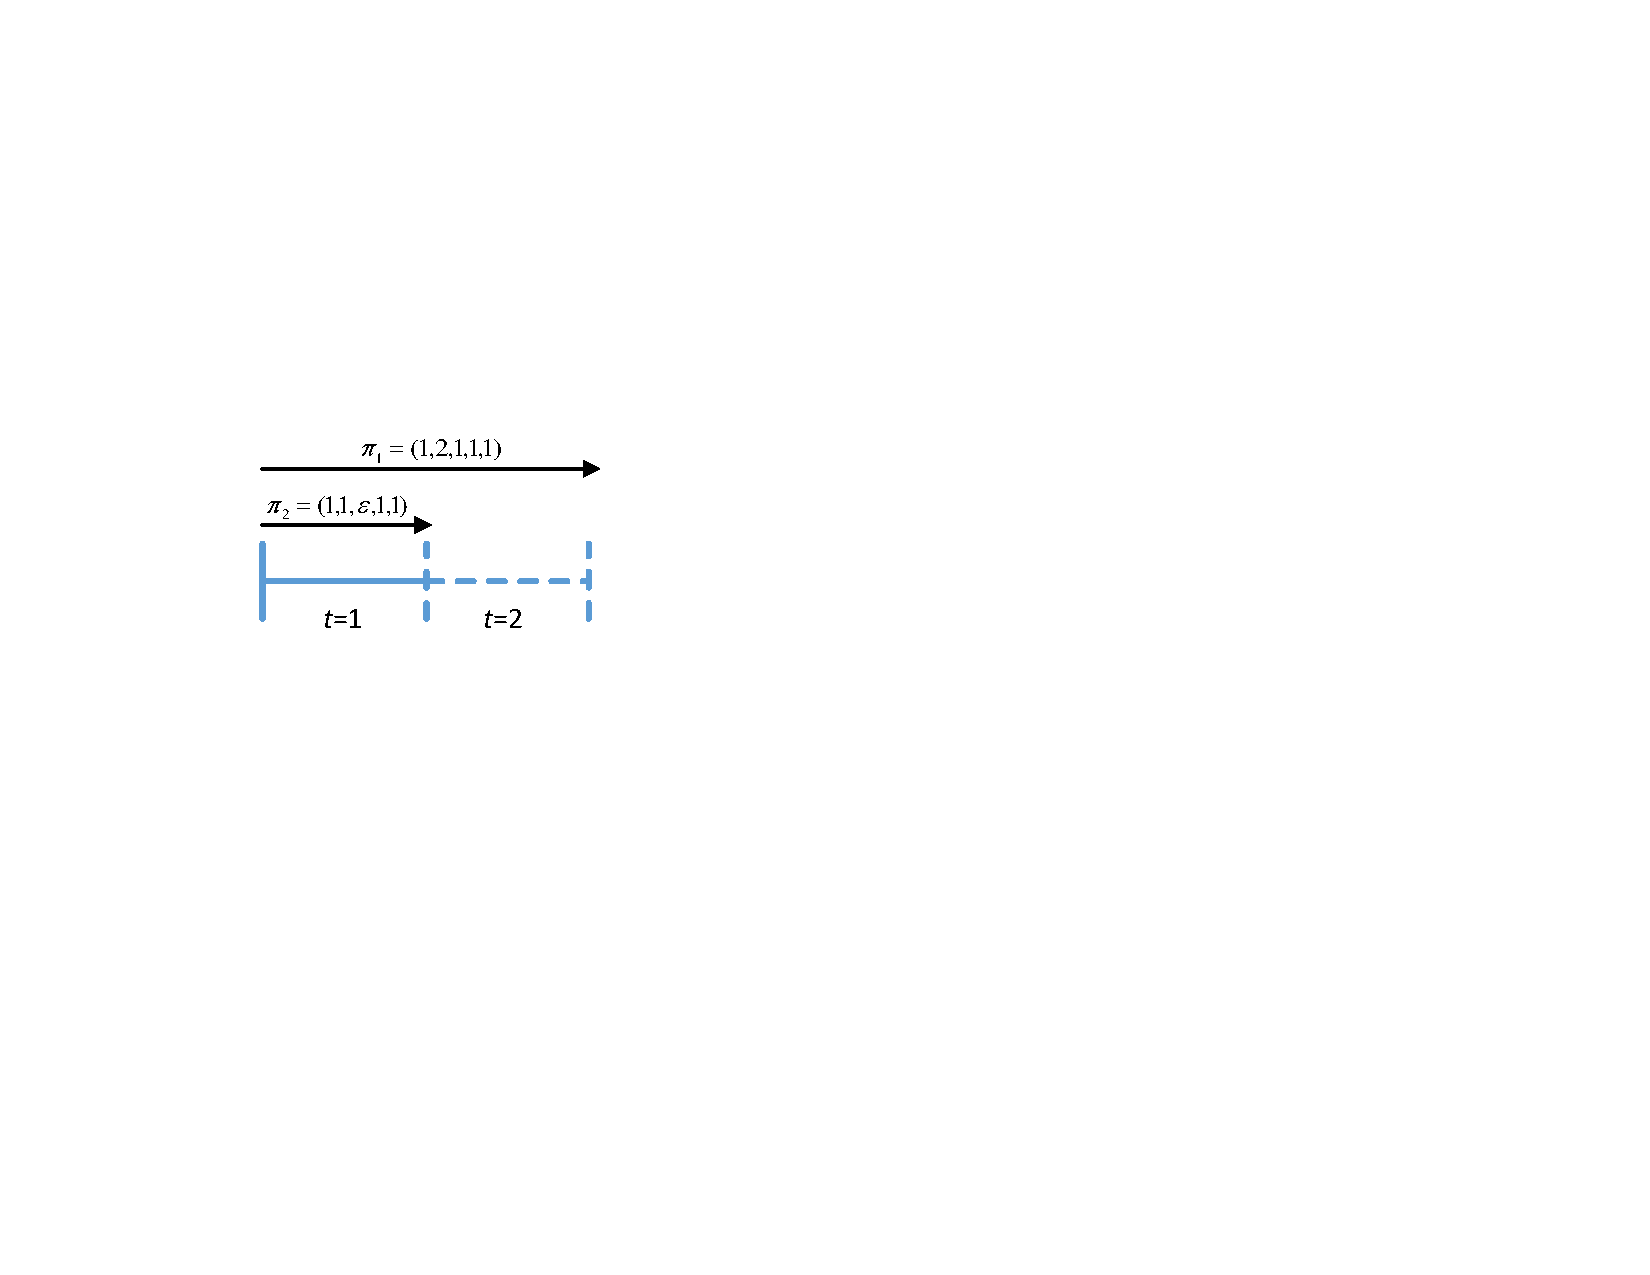
\includegraphics[width=60mm]{Ex1a.pdf}}
		\hspace{8mm}
		\subfloat[{EV $3$ arrives at $t=2$.}]{\label{fig:1b}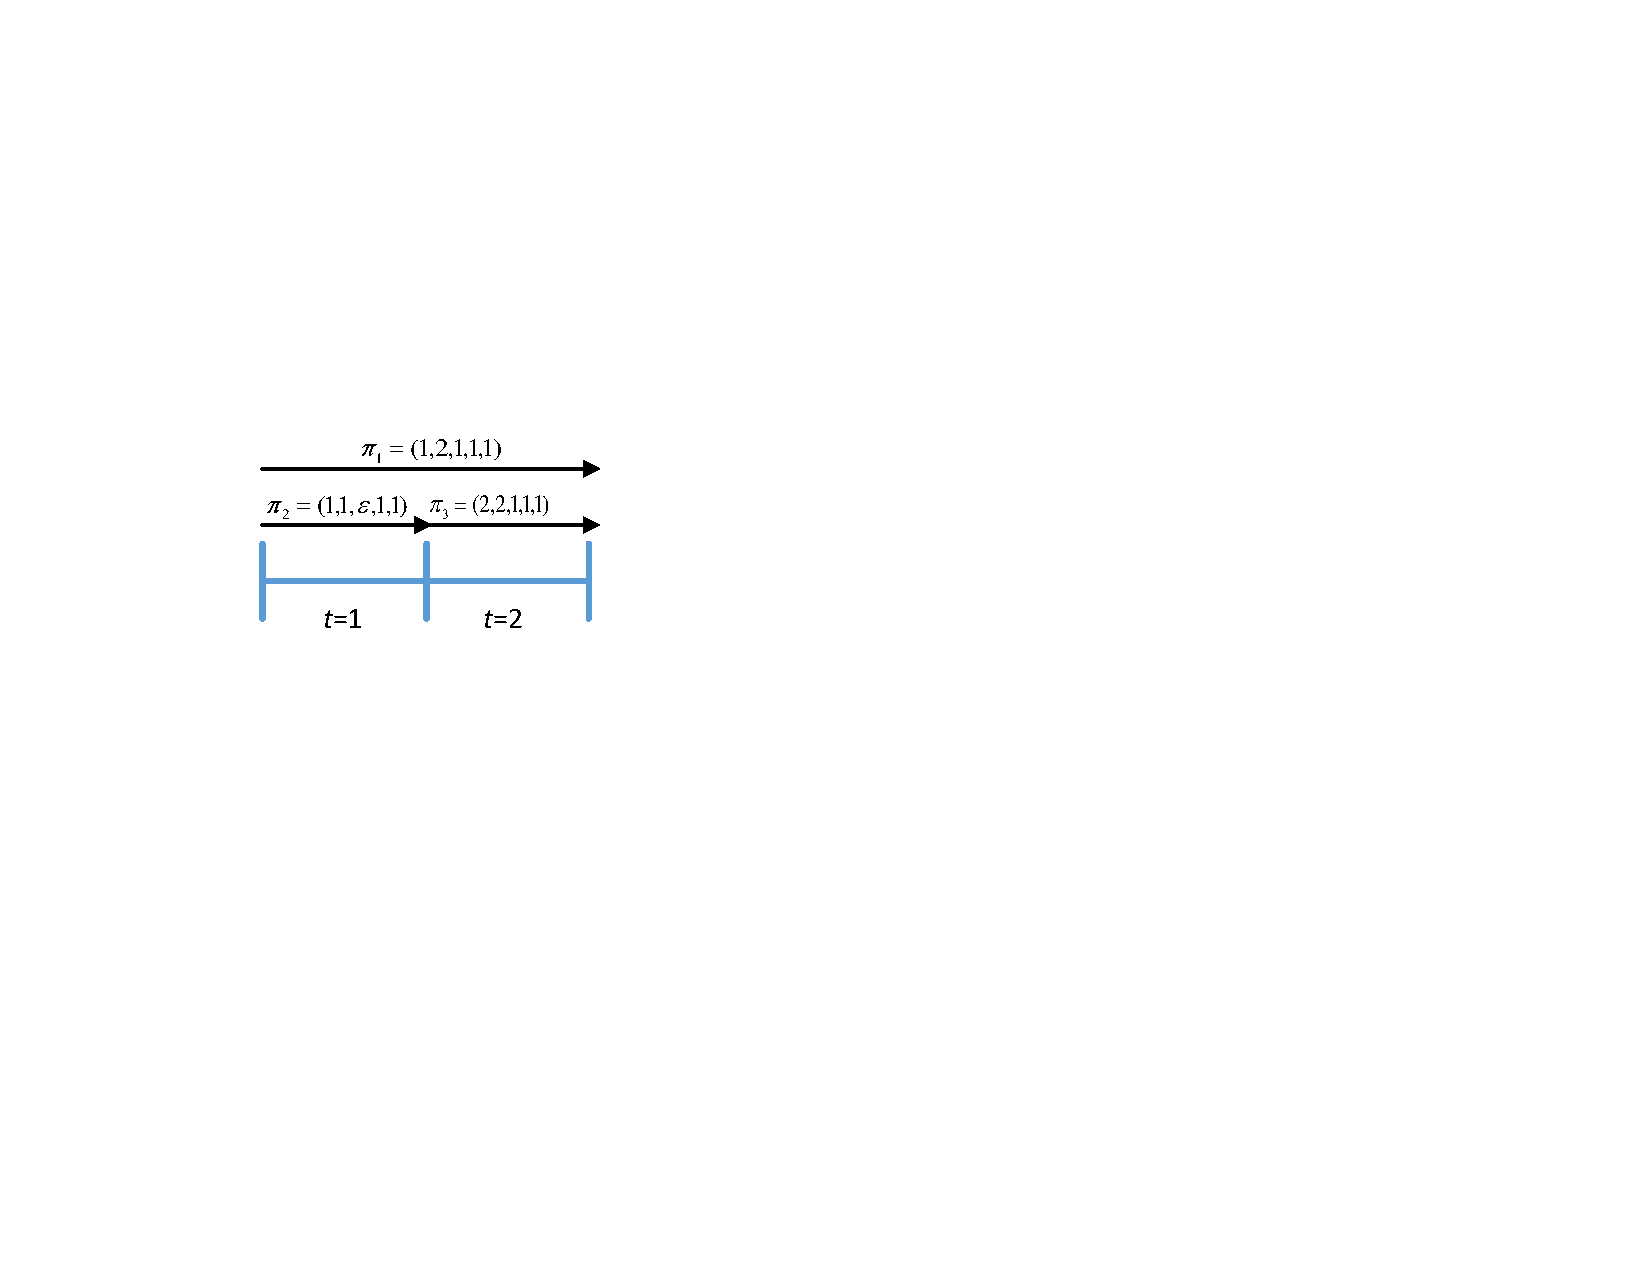
\includegraphics[width=60mm]{Ex1b.pdf}}
\caption{Worst case scenario when the scheduling algorithm is to re-run an optimal algorithm at each time slot considering only available EVs. Dotted line indicates a time slot that is not visited yet and the scheduler has no information about the arriving EVs in that slot. The numbers inside parentheses indicate arrival time, deadline, value, demand and maximum charging rate of the EV, respectively.}
\label{fig:1}
\end{figure}

\vspace{3mm}
{\color{blue} In the experimental evaluation the results for both models are put together in the same figure, which gets us into the odd situation that some results are better than optimal.
 }
\vspace{3mm}

$\vartriangleright$ \noindent\textbf{Response:} 
We agree and this is unfortunately consequence of space limit. To avoid confusion, we added an explanation in Page xx, when describing the results. 

\vspace{3mm}
{\color{blue} typos:
p3: "We formulate Scheduling"

p3:l33: "ptotal, which we refer to it as the global peak, hereafter" => I think you mean to say that this is the capacity limit, not the global peak.

p4: "a definitions"

p7: "If there is not enough resources"

p7: "In primal-dual algorithm"

note [page 8]: Other approximations?

p8: "under integral mode"

p8: "for fractional mode"

p8: "We propose the IOCS"

p8: "over set of"

p8: "with optima"

p8: "in accordance to NHTS survey"

p8: "of arriving an EV in the peak hours"

p9: "in integral revenue

p9: "The proposed algorithms compared to"

p9: "IO LP.Recall"
 }
\vspace{3mm}

$\vartriangleright$ \noindent\textbf{Response:} 
...


\begin{itemize}
\item B. Alinia, M. S. Talebi, M. H. Hajiesmaili, A. Yekkehkhany and N. Crespi, Competitive Online Scheduling Algorithms with Applications in Deadline-Constrained EV Charging, IEEE/ACM 26th International Symposium on Quality of Service (IWQoS), 2018
doi: 10.1109/IWQoS.2018.8624184

\item de Weerdt, M. M., Albert, M., Conitzer, V., \& Linden, K. V. D. (2018). Complexity of scheduling charging in the smart grid. In Proceedings of the Twenty-Seventh International Joint Conference on Artificial Intelligence (pp. 4736-4742).

\item Yao, L., Lim, W. H., \& Tsai, T. S. (2017). A real-time charging scheme for demand response in electric vehicle parking station. IEEE Transactions on Smart Grid, 8(1), 52-62.
\end{itemize}

\newpage
\section{Reviewer $\# 2$}

\vspace{3mm}
{\color{blue} 1.      The authors need to examine the literature more thoroughly. Although the proposed methods have a certain degree of novelty, more related works exist. For example, the authors could consider some of the following papers, while others may also exist.

\begin{itemize}
\item a: Huang, S., Wu, Q., Oren, S. S., Li, R., \& Liu, Z. (2015). Distribution locational marginal pricing through quadratic programming for congestion management in distribution networks. IEEE Transactions on Power Systems, 30(4), 2170-2178.

\item b: Hu, J., You, S., Lind, M., \& Østergaard, J. (2014). Coordinated charging of electric vehicles for congestion prevention in the distribution grid. IEEE Transactions on Smart Grid, 5(2), 703-711.

\item c: Rigas, E. S., Ramchurn, S. D., Bassiliades, N., \& Koutitas, G. (2013, October). Congestion management for urban EV charging systems. In 2013 IEEE International Conference on Smart Grid Communications (SmartGridComm) (pp. 121-126). IEEE.

\end{itemize}
}
\vspace{3mm}

$\vartriangleright$ \noindent\textbf{Response:} 
Thanks for suggesting the related works. In the revised version we added all of them as well as several more recent papers, that are highlighted in blue. 

{\color{red} I should check these papers and add to Related Work if needed.}

\vspace{3mm}
{\color{blue} 2. The authors claim that if prediction or modeling techniques were used, the performance of the proposed algorithms would deteriorate. However, they do not present any results to support their claim.  }
\vspace{3mm}

$\vartriangleright$ \noindent\textbf{Response:} 
This refers to the following statement in the Related Work: "The prediction-based approaches achieve satisfactory performance for the scenarios that follow prediction. Deviation from prediction models, however, degrades their performance.
Our approach, on the other hand, has no assumptions on modeling/prediction, and in this way, is robust against any uncertainty in the instances to the problem." 

The above statement provides a high-level difference between prediction-based approaches and our competitive online algorithm design approach. Since our approach does not rely on any predicted future information, we are robust against any type of uncertain input to the problem. In contrast, the developed algorithms in prediction-based approaches rely on the quality of prediction, and if the quality of prediction is weak, their performance also degrades. An interesting future direction of our work, based on this comment, is to extend our \textit{pure} online algorithms with a limited predicted future values. In this way, not only the algorithms are robust against uncertainty, their performance in practice can be improved with some future data. 

\vspace{3mm}
{\color{blue} 3. An interesting extension would be to let users define a set of CSs to charge and let the scheduling algorithms take the final decision of the CS to charge. In this way, the flexibility of the algorithms would increase and the load across the CSs could be better managed. However, the downside would be that the complexity of the algorithms would increase. }
\vspace{3mm}

$\vartriangleright$ \noindent\textbf{Response:} 
Although this can be an interesting extension, in this version, we assumed that a user chooses only one CS to ask for its demand and may drive to another CS if its demand is not fulfilled. We admit that this suggestion is a very elegant extension from the perspective of theoretical problem formulation and algorithm design, and makes the scenario more challenging. In addition, this suggestion makes more sense in scenarios in which EVs are heterogeneous and a subset of chargers can satisfy a subset of EVs. We do believe that this is an very interesting scenario to consider, however, as mentioned by the reviewer, it increases the complexity of designing and analysis of the algorithms, and is beyond the scope of this submission. 

\vspace{3mm}
{\color{blue} Is truth telling regarding the EVs’ valuations guaranteed? Is it possible for the EVs to cooperate and report lower valuations? It is not clear in the paper. If not, this could come in contrast with the revenue maximization objective function. Moreover, this would cause serious implications in the online algorithms which use the valuations to select the EVs to charge.}
\vspace{3mm}

$\vartriangleright$ \noindent\textbf{Response:} 
This is an important and interesting point raised by the reviewer. Although we did not study the case for self interested users in this paper, we addressed it in our recent work: 

B. Alinia, M. H. Hajiesmaili, and N. Crespi, "Online EV Charging Scheduling with On-Arrival Commitment", \textit{IEEE Trans. on Int. Transportation Systems (ITS)}, 2019.

In the above cited paper, we propose "SCOMMIT" algorithm where its core allocation idea is based on users' unit-values except that it also provides on-arrival commitment. Since it is proved that SCOMMIT is truthful, we believe that among the proposed algorithms in current manuscript, the FOCS is truthful. In the above paper, also, we tackled another desirable property to commit EVs on their arrival on how much they can get charged during their available window. 

The focus of this paper, in on more comprehensive online algorithm design for fractional and integral revenue models, and for our ITS paper, we focused on truthfulness and on-arrival commitment. It is worth noting that developing solutions that provide competitiveness against offline optimal versus those that provide truthfulness and on-arrival commitment, needs different algorithmic techniques and tools. As a notable result, an interesting theoretical observation in our ITS shows that there is no online algorithms that can simultaneously provide on-arrival commitment and bounded competitive ratio. See Section 6 and Theorem 5 of our ITS paper for more details. 

\vspace{3mm}
{\color{blue} 5. The length of each time point is set to 1 hour. This is too long, and the accuracy of the algorithms is reduced. Moreover, the online algorithm is not really online, as it schedules EVs every hour. }
\vspace{3mm}

$\vartriangleright$ \noindent\textbf{Response:} 
The length of the time slot can be arbitrary set in the algorithms and we used 1 hour in experiments since the availability window of our traces was in one hour slots. With more fine grained data, it would be possible to run the algorithms in faster timescales, e.g., 5 minutes or so. 

We note that the derived complexities of the algorithms in the paper include parameter $T$ as number of time slots in a day (please see Table II in the manuscript). In large scale scenarios, the effect of increasing $T$ would be negligible in performance of the algorithms as long as it $T/N$ is a constant ($N$ is number of EVs). Therefore, when $N$ grows large and $T$ is a constant, $T$ can be removed from the complexities in the Table II. 

%Another point is that in real electricity market prices are only allowed to be changed hourly which is the reason most power scheduling algorithms work with one-hour slots.

\vspace{3mm}
{\color{blue} Some results on execution times and scalability of the proposed algorithms must be added.
 }
\vspace{3mm}

$\vartriangleright$ \noindent\textbf{Response:} 
The complexity of the algorithms are low and we just set the charging rate by a simple sorting on arrival of each EV. \textbf{Bahram, please confirm.}

%\bibliography{ref-response}{}
%\vspace{-3mm}
%\bibliographystyle{ieeetr}

\end{document}